% !TEX program = xelatex
% !TEX encoding = UTF-8 Unicode
%
% SPDX-License-Identifier: CC-BY-4.0
% Wei JungYing, Wu KunChe, Zheng YiKai

% Use 16:9 aspect ratio (required for this course)
\documentclass[aspectratio=169]{beamer}
\mode<presentation>{
    \usetheme{NordlingLab169}
}

% Load packages
\usepackage[english]{babel}
\let\latinencoding\relax
\usepackage{xltxtra}
% Use a system font (Candara is the official font, but may not be available)
% Alternatives: Helvetica Neue (macOS), DejaVu Sans (Linux), Calibri (Windows)
% Uncomment the appropriate font for your system:
% \setsansfont{Helvetica Neue}[BoldFont = Helvetica Neue Bold, ItalicFont = Helvetica Neue Italic]  % macOS
% \setsansfont{DejaVu Sans}[BoldFont = DejaVu Sans Bold, ItalicFont = DejaVu Sans Oblique]  % Linux
\setsansfont{Calibri}[BoldFont = Calibri Bold, ItalicFont = Calibri Italic]  % Windows

\usepackage{graphicx}
\usepackage[yyyymmdd]{datetime}
\renewcommand{\dateseparator}{--}
\usepackage{booktabs}
\usepackage{amsmath}

% Presentation metadata
\title[Drowsiness Detection]{Driver Drowsiness Detection System}
\subtitle{ECG-based Fatigue Analysis with Multi-Agent AI Architecture}
\author[Wei, Wu, Zheng]{Wei,~JungYing \and Wu,~KunChe \and Zheng,~YiKai}
\institute[NCKU]{
    National Cheng Kung University\\
    Agentic AI Course -- Spring 2026
}
\date{\today}
\subject{Driver Drowsiness Detection using ECG and Agentic AI}

\begin{document}

% ============================================
% SLIDE 1: TITLE
% ============================================
\setbeamertemplate{background}[NLTitle]
\setbeamertemplate{footline}[NLTitle]
\begin{frame}
    \titlepage
\end{frame}

% ============================================
% SLIDE 2: OUTLINE
% ============================================
\setbeamertemplate{background}[NLCC]
\setbeamertemplate{footline}[NLCC]
\begin{frame}{Outline}
    \tableofcontents
\end{frame}

% ============================================
% SECTION: PROBLEM & MOTIVATION
% ============================================
\section{Problem \& Motivation}

% ============================================
% SLIDE 3: PROBLEM STATEMENT
% ============================================
\begin{frame}{Problem Statement}
    \begin{columns}
        \begin{column}{0.6\textwidth}
            \textbf{Driver Fatigue: A Critical Safety Issue}
            \begin{itemize}
                \item Driver fatigue causes \textbf{thousands of accidents} globally each year
                \item Alert-to-drowsy transition is \textbf{invisible} to the driver
                \item Delayed reaction time and impaired decision-making
                \item Current solutions have significant limitations:
                \begin{itemize}
                    \item Camera-based: Fails in poor lighting
                    \item Steering-based: Detects too late
                \end{itemize}
            \end{itemize}
        \end{column}
        \begin{column}{0.35\textwidth}
            \centering
            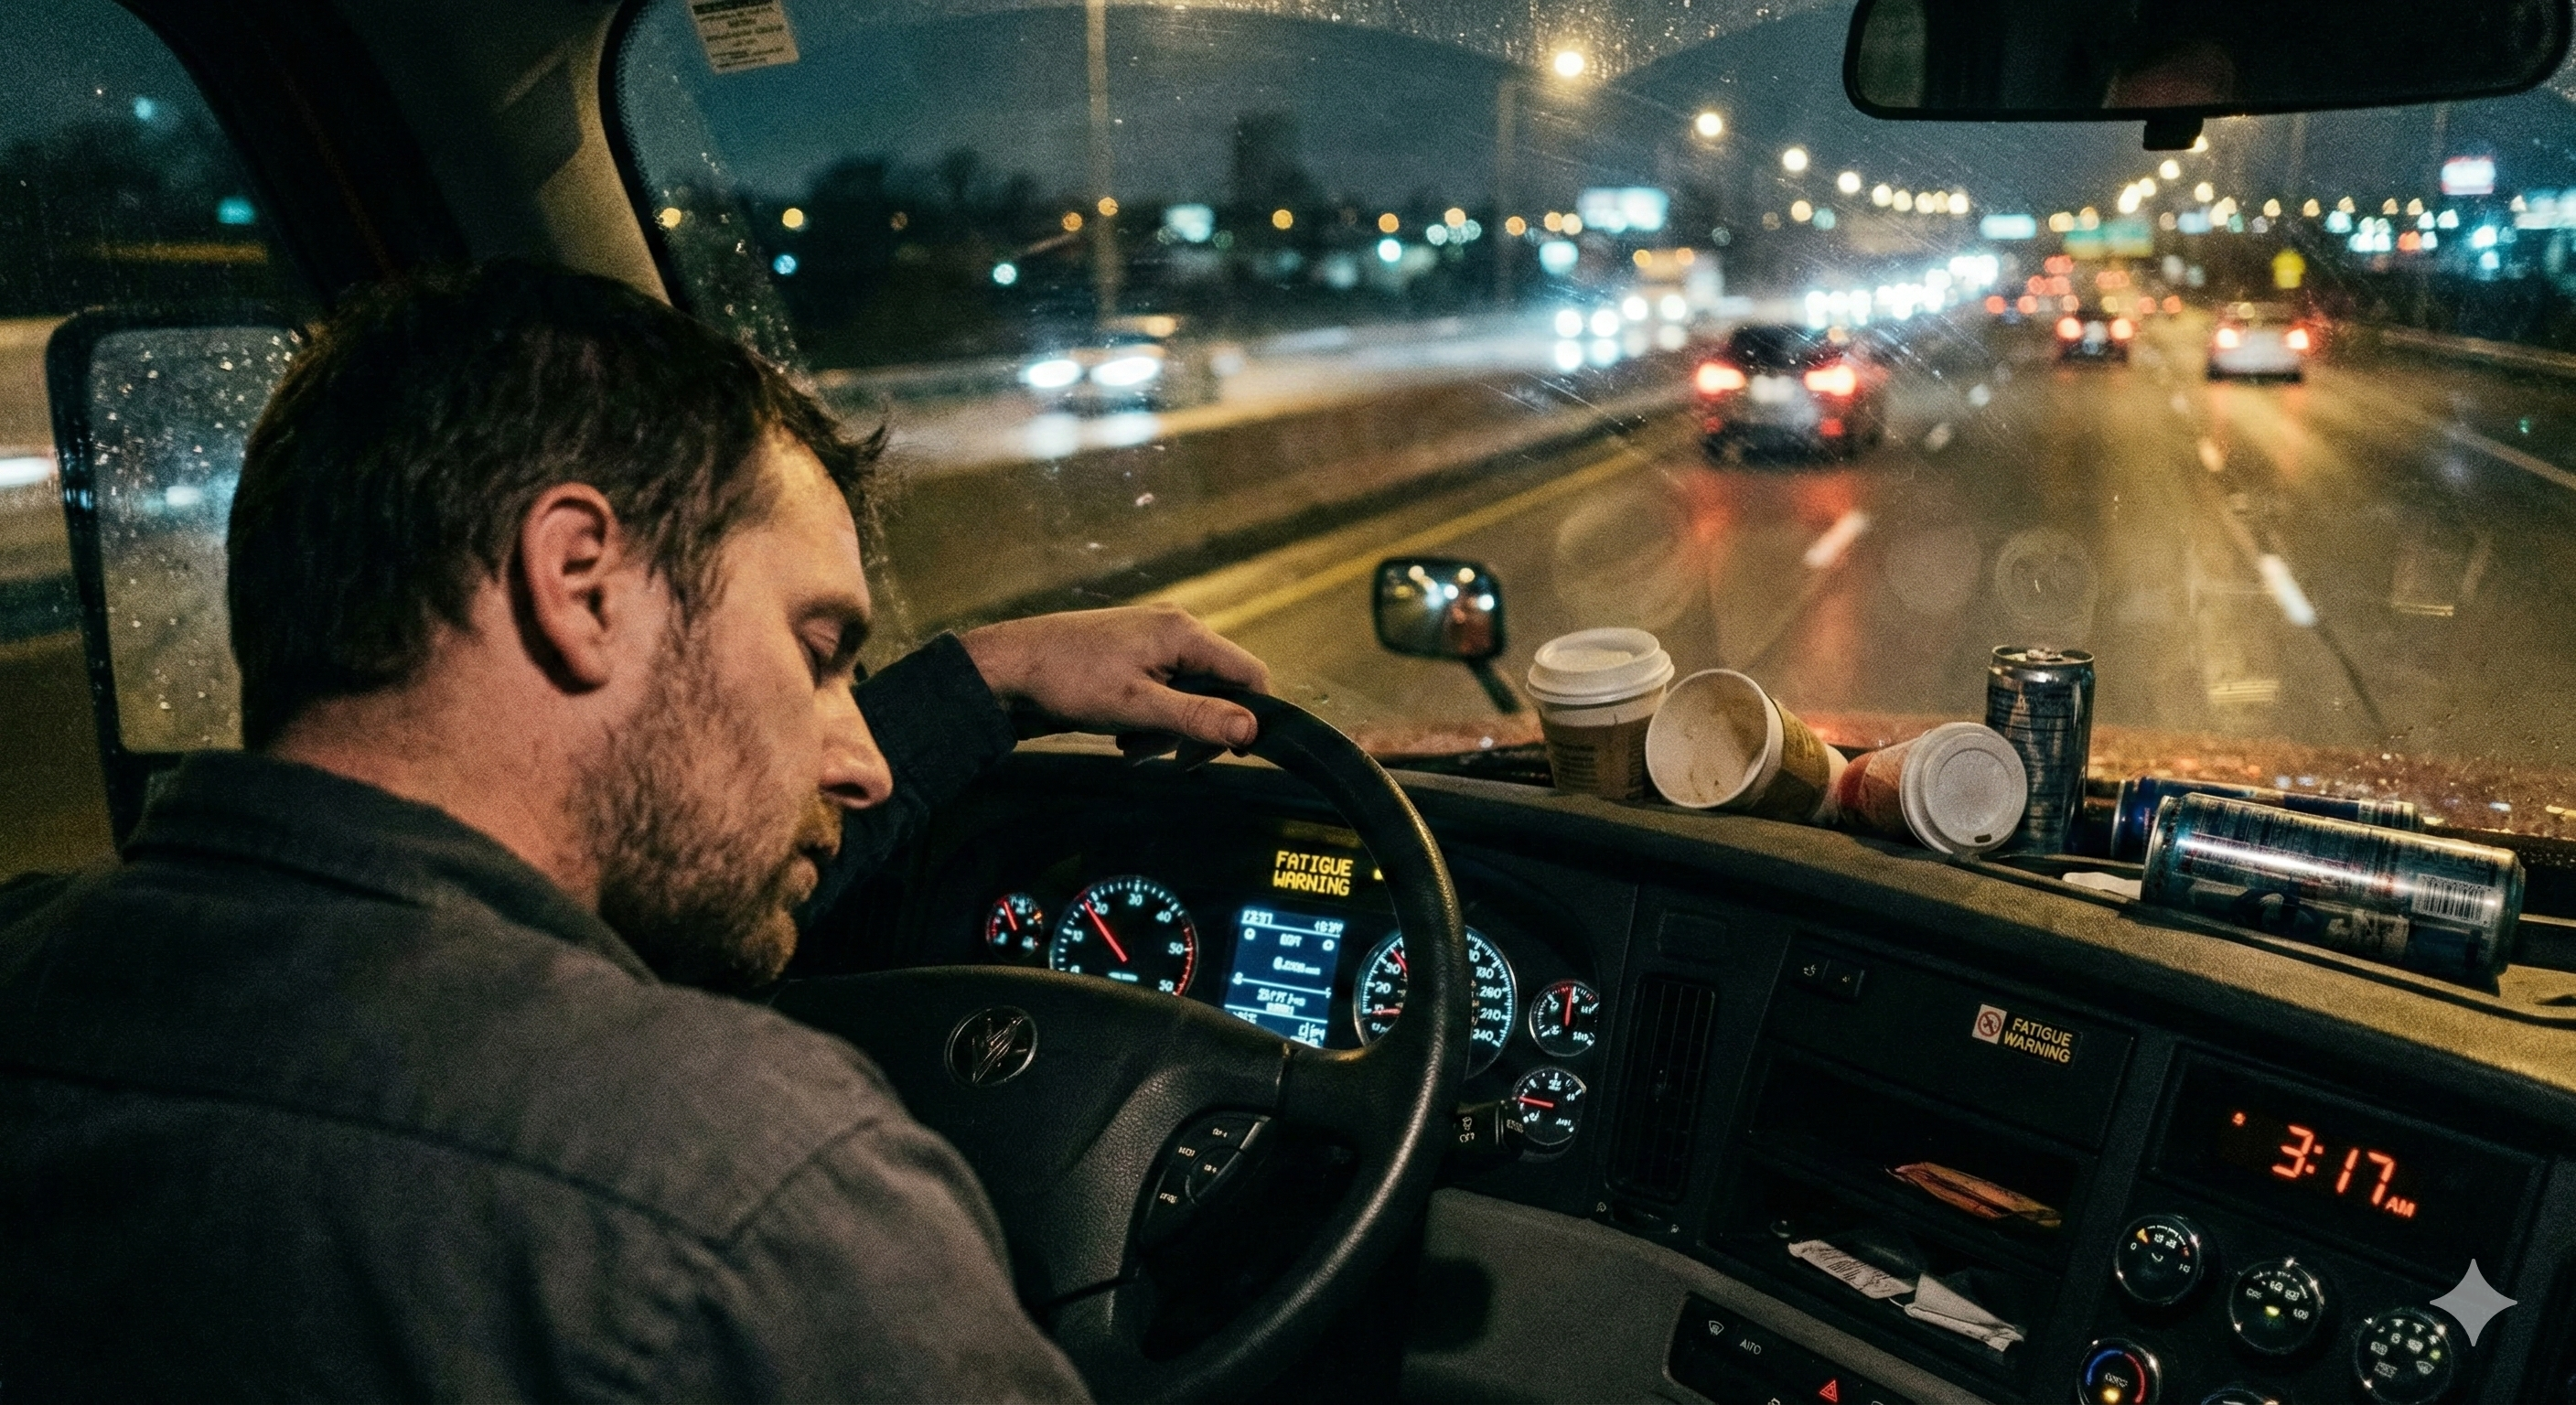
\includegraphics[width=\textwidth]{2026-Wei-Wu-Zheng-drowsy-driver.png}
        \end{column}
    \end{columns}
\end{frame}

% ============================================
% SLIDE 4: OUR SOLUTION
% ============================================
\begin{frame}{Our Solution: ECG-based Detection}
    \textbf{Why ECG?}
    \begin{itemize}
        \item \textbf{Physiological indicator}: Directly measures autonomic nervous system activity
        \item \textbf{Continuous monitoring}: Non-invasive, works in all conditions
        \item \textbf{Early detection}: Changes in HR and HRV precede behavioral signs
    \end{itemize}

    \vspace{1em}
    \textbf{Key Physiological Markers:}
    \begin{table}
        \centering
        \begin{tabular}{lcc}
            \toprule
            \textbf{Metric} & \textbf{Alert State} & \textbf{Drowsy State} \\
            \midrule
            Heart Rate (HR) & Higher (70-80 bpm) & Lower (55-65 bpm) \\
            HRV (SDNN) & Lower (30-50 ms) & Higher (70-100 ms) \\
            \bottomrule
        \end{tabular}
    \end{table}
\end{frame}

% ============================================
% SECTION: SYSTEM ARCHITECTURE
% ============================================
\section{System Architecture}

% ============================================
% SLIDE 5: THREE-AGENT ARCHITECTURE
% ============================================
\begin{frame}{Three-Agent Agentic AI Architecture}
    \begin{columns}
        \begin{column}{0.55\textwidth}
            \centering
            \includegraphics[width=\textwidth]{2026-Wei-Wu-Zheng-architecture.pdf}
        \end{column}
        \begin{column}{0.43\textwidth}
            \textbf{Agent 1 - Signal Filter:}
            \begin{itemize}
                \item Bandpass filter (0.5-40 Hz)
                \item Notch filter, Normalization
            \end{itemize}

            \textbf{Agent 2 - Feature Extraction:}
            \begin{itemize}
                \item R-peak detection
                \item HR, HRV metrics (SDNN, RMSSD)
            \end{itemize}

            \textbf{Agent 3 - Decision + MCP:}
            \begin{itemize}
                \item Multi-factor risk scoring
                \item MCP tool queries
            \end{itemize}
        \end{column}
    \end{columns}
\end{frame}

% ============================================
% SLIDE 6: MCP TOOL INTEGRATION
% ============================================
\begin{frame}{MCP Tool Integration for Contextual Awareness}
    \textbf{Model Context Protocol (MCP) Tools}

    \vspace{0.5em}
    Agent 3 queries multiple contextual factors:

    \vspace{0.5em}
    \begin{columns}
        \begin{column}{0.48\textwidth}
            \begin{block}{Environmental Context}
                \begin{itemize}
                    \item \textbf{Weather Query}: Hot/humid $\rightarrow$ higher fatigue
                    \item \textbf{Time Risk}: 02:00-05:00 = Very High risk
                    \item \textbf{Rest Areas}: Nearest rest stops
                \end{itemize}
            \end{block}
        \end{column}
        \begin{column}{0.48\textwidth}
            \begin{block}{Driver Context}
                \begin{itemize}
                    \item \textbf{Driving Duration}: $>$2 hours = High risk
                    \item \textbf{Medical KB}: HRV interpretation
                    \item \textbf{Personal Baseline}: Individual variation
                \end{itemize}
            \end{block}
        \end{column}
    \end{columns}

    \vspace{1em}
    \centering
    \textit{Multi-modal integration for more accurate drowsiness detection}
\end{frame}

% ============================================
% SECTION: DEMO & RESULTS
% ============================================
\section{Demo \& Results}

% ============================================
% SLIDE 7: RISK SCORING SYSTEM
% ============================================
\begin{frame}{Risk Scoring System}
    \textbf{Multi-Factor Risk Assessment}

    \vspace{0.5em}
    \begin{table}
        \centering
        \begin{tabular}{lc}
            \toprule
            \textbf{Risk Factor} & \textbf{Max Score} \\
            \midrule
            Low Heart Rate ($<$60 bpm) & 30 \\
            High HRV (SDNN $>$ 80 ms) & 35 \\
            Baseline Deviation & 15 \\
            Time Risk (late night) & 40 \\
            Weather Factors (hot/humid) & 15 \\
            Driving Duration ($>$3 hours) & 40 \\
            \midrule
            \textbf{Maximum Total} & \textbf{175} \\
            \bottomrule
        \end{tabular}
    \end{table}

    \vspace{0.5em}
    \textbf{Risk Levels:} Low (0-29) | Medium (30-49) | High (50-69) | Very High (70+)
\end{frame}

% ============================================
% SLIDE 8: TEST RESULTS
% ============================================
\begin{frame}{Test Results}
    \textbf{Validation with Synthetic ECG Data}

    \vspace{0.5em}
    \begin{table}
        \centering
        \begin{tabular}{lccc}
            \toprule
            \textbf{Test Data} & \textbf{Expected} & \textbf{Actual} & \textbf{Status} \\
            \midrule
            ecg\_normal.csv & Low Risk & Low Risk & \textcolor{green}{PASS} \\
            ecg\_drowsy.csv & High Risk & Very High & \textcolor{green}{PASS} \\
            ecg\_long\_drowsy.csv & Very High & Very High & \textcolor{green}{PASS} \\
            \bottomrule
        \end{tabular}
    \end{table}

    \vspace{1em}
    \textbf{Performance Metrics:}
    \begin{itemize}
        \item Test suite: \textbf{25 tests, 100\% pass rate}
        \item Processing time: \textbf{$<$1 second} for 30-second recording
        \item Pipeline latency: \textbf{$<$2 seconds} end-to-end
    \end{itemize}
\end{frame}

% ============================================
% SLIDE 9: LIVE DEMO (SCREENSHOT)
% ============================================
\begin{frame}{System Interface}
    \centering
    \textbf{Streamlit Web Application}

    \vspace{0.5em}
    
    \includegraphics[width=0.85\textwidth]{2026-Wei-Wu-Zheng-screenshot.png}

    \vspace{0.5em}
    \footnotesize{\textit{Figure: Real-time driver fatigue monitoring dashboard}}
\end{frame}

% ============================================
% SECTION: CHALLENGES & LESSONS
% ============================================
\section{Challenges \& Lessons Learned}

% ============================================
% SLIDE 10: CHALLENGES
% ============================================
\begin{frame}{Challenges \& Solutions}
    \begin{columns}
        \begin{column}{0.48\textwidth}
            \textbf{Technical Challenges:}
            \begin{enumerate}
                \item \textbf{Motion Artifacts}
                \begin{itemize}
                    \item Solution: Multi-stage filtering
                \end{itemize}
                \item \textbf{Individual Variation}
                \begin{itemize}
                    \item Solution: Personalized baseline
                \end{itemize}
                \item \textbf{Real-time Processing}
                \begin{itemize}
                    \item Solution: Efficient signal processing
                \end{itemize}
            \end{enumerate}
        \end{column}
        \begin{column}{0.48\textwidth}
            \textbf{Lessons Learned:}
            \begin{enumerate}
                \item \textbf{Agent modularity} enables independent testing and improvement
                \item \textbf{MCP tools} provide valuable context beyond physiological data
                \item \textbf{Rule-based decisions} can be effective without API costs
            \end{enumerate}
        \end{column}
    \end{columns}
\end{frame}

% ============================================
% SLIDE 11: AGENTIC VS CHAT-BASED
% ============================================
\begin{frame}{Agentic AI vs Chat-based Approach}
    \begin{table}
        \centering
        \begin{tabular}{lcc}
            \toprule
            \textbf{Aspect} & \textbf{Agentic AI} & \textbf{Chat-based} \\
            \midrule
            Processing Time & 1-2 seconds & 30-45 minutes \\
            Manual Steps & 1 (upload file) & 10+ steps \\
            Error Rate & 0\% (automated) & Higher (manual) \\
            Reproducibility & 100\% & Variable \\
            Real-time Capable & Yes & No \\
            \bottomrule
        \end{tabular}
    \end{table}

    \vspace{1em}
    \textbf{Key Insight:} Agentic AI excels at \textbf{repetitive, multi-step workflows} with clear structure. Chat-based AI is better for \textbf{exploratory, one-off questions}.
\end{frame}

% ============================================
% SECTION: CONCLUSION
% ============================================
\section{Conclusion}

% ============================================
% SLIDE 12: CONCLUSION & Q&A
% ============================================
\begin{frame}{Conclusion}
    \textbf{Summary:}
    \begin{itemize}
        \item Built a \textbf{three-agent pipeline} for ECG-based drowsiness detection
        \item Integrated \textbf{MCP tools} for multi-modal context awareness
        \item Achieved \textbf{100\% test pass rate} with $<$2s processing time
        \item Demonstrated clear advantages over chat-based approaches
    \end{itemize}

    \vspace{1em}
    \textbf{Future Work:}
    \begin{itemize}
        \item Integrate real weather API and GPS location
        \item Validate with real ECG data from driving studies
        \item Add real-time streaming support
    \end{itemize}

    \vspace{1.5em}
    \centering
    \Large{\textbf{Thank you! Questions?}}

    \vspace{0.5em}
    \normalsize{Code: \texttt{project-code-group/2026-Wei-Wu-Zheng/}}
\end{frame}

\end{document}
